\chapter{Métodos perturbativos}
Comenzamos el estudio de los métodos perturbativos por las
perturbaciones estacionarias. En ellas tenemos fuerzas no dependientes
del tiempo actuando sobre el sistema.

Escribimos el hamiltoniano del sistema como la suma de un hamiltoniano
sin perturbar $ \Ham _0$ y una perturbación $W$ despreciable:
\begin{equation}
   \Ham  =  \Ham _0 + W 
\end{equation}
No estamos comparando energías, sino operadores, lo que dificulta
identificar cuando $W$ es realmente despreciable.

Suponemos que para $ \Ham _0$ conocemos la solución a la ecuación de
autovalores:
\begin{equation}
   \Ham _0 \ket{\varphi_p^i} = E_p \ket{\varphi_p^i}
\label{eq:originalH}
\end{equation}
donde $p$ es el índice que indexa los distintos autovectores y $i$ el
índice para diferenciar soluciones en caso de existir degeneración.
Utilizaremos los $\ket{\varphi_p^i}$ como base del espacio.

Escribimos $W=\lambda \hat{W}$ de forma que podamos ``regular'' el
efecto de la perturbación con el factor escalar $\lambda$, con lo que
obtenemos $ \Ham (\lambda) =  \Ham _0 + \lambda\hat{W} $.
Nos queda
\begin{equation}
   \Ham  \varphi(\lambda) = E(\lambda)\varphi(\lambda)
\label{eq:lambdaschr}
\end{equation}
Tratamos de hallar la $E(\lambda)$. Si la perturbación no es muy
grande, es de suponer que $\{E(\lambda)\} \sim \{E_p\}$. 

Utilizando series de potencias:
\begin{align}
  E(\lambda) &= \varepsilon_0 + \varepsilon_1 \lambda + \varepsilon_2 \lambda^2
  + \cdots \\
  \varphi(\lambda) &= \ket{0} + \lambda \ket{1} + \lambda^2 \ket{2} 
  + \cdots 
                  \label{eq:varphilamb}
\end{align}
Escribimos la ecuación de Schrödinger \eqref{eq:lambdaschr}:
\begin{equation}
  ( \Ham _0 + \lambda \hat{W})[\ket{0} + \lambda \ket{1} +
  \cdots] = \left( \sum_{i=1}^\infty \varepsilon_i \lambda^i  \right)
  \left( \sum_{i=1}^\infty \lambda^i \ket{i}  \right)
\end{equation}
Igualamos las distintas potencias de $\lambda$:
\begin{equation}
  \begin{split}
    \lambda^0 &:\ \  \Ham _0 \ket{0} = \varepsilon_0 \ket{0} \\
    \lambda^1 &:\ \  \Ham _0 \ket{1} + \hat{W} \ket{0} =
    \varepsilon_0 \ket{1}+ \varepsilon_1 \ket{0} \\
    \lambda^2 &:\ \  \Ham _0 \ket{2} + \hat{W} \ket{1} =
    \varepsilon_0 \ket{2} +\varepsilon_1 \ket{1} + \varepsilon_2 \ket{0} \\
    \cdots & \\
    \lambda^q &:\ \  \Ham _0 \ket{q} + \hat{W} \ket{q-1} =
    \varepsilon_0 \ket{q}+ \varepsilon_1 \ket{q-1} + \cdots + \varepsilon_q \ket{0} \\
  \end{split}
\end{equation}
A partir de orden 1 (lineal) se suele cortar la aproximación, ya que
no merece la pena precisar más por ser probablemente los $E_p$ usados
fruto de una aproximación.

Sabemos que \eqref{eq:lambdaschr} determina $\varphi(\lambda)$ sólo salvo
un factor de fase, lo que nos permite elegir la norma de
$\varphi(\lambda)$ y su fase. Escogemos que $\varphi(\lambda)$ esté
normalizado y tenga una fase tal que $\braket{0}{\varphi} \in
\mathbb{R}$. Utilizando esto en la ecuación \eqref{eq:varphilamb} surgen
varias consecuencias:
\begin{itemize}
\item En orden de aproximación nulo\footnote{ Si $\varphi(\lambda) \sim
    \ket{0}$ se obtiene
    \begin{equation*}
      \abs{\varphi(\lambda)}^2 = \braket{0}{0} = 1
    \end{equation*}
}, el ket $\ket{0}$ ha de estar
  normalizado.
\begin{equation}
  \braket{0}{0} =1
\end{equation}
\item A primer orden\footnote{Ahora $\varphi(\lambda)\sim \ket{0} +
    \lambda \ket{1}$ y se obtiene
    \begin{equation*}
      \begin{split}
        \abs{\varphi(\lambda)}^2 &= (\bra{0} + \lambda\bra{1})(\ket{0} +
        \lambda\ket{1}) = \\
        &= \cancelto{1}{\ip{0}} + \lambda\braket{0}{1} + \\ &+ \lambda\braket{1}{0} +
        \order{\lambda^2} = \\
        &= \cancel{1}
      \end{split}
    \end{equation*}
    Por lo que $\braket{0}{1}$ ha de ser igual a $-\braket{1}{0}$ y
    por tanto deben ser nulos.
    }, vemos que los kets $\ket{0}$ y $\ket{1}$ son
  perpendiculares:
\begin{equation}
  \braket{0}{1} = \braket{1}{0} = 0
\end{equation}
\item En segundo orden\footnote{
Las ecuaciones se complican, pero descartando términos
$\order{\lambda^3}$ y superiores se obtiene
\begin{equation*}
  \begin{split}
    \abs{\varphi(\lambda)}^2 
    &= \cancelto{1}{\ip{0}} + \cancelto{0}{\lambda\braket{0}{1}} + \lambda^2 \braket{0}{2} + \\
    &+  \cancelto{0}{\lambda\braket{1}{0}} + \lambda^2 \braket{1}{1} +
    \lambda^2 \braket{2}{0} = \\ &= \cancel{1}
  \end{split}
\end{equation*}
 Obtenemos que $\braket{2}{0} + \braket{0}{2} = -\braket{1}{1}$, y
 utilizando el convenio $\braket{2}{0} = \braket{0}{2}$ para las fases
 (puramente reales) se obtiene la ecuación \eqref{eq:captainamerica}.
},
\begin{equation}
  \braket{0}{2} = \braket{2}{0} = - \frac{1}{2} \braket{1}{1}
  \label{eq:captainamerica}
\end{equation}
\item En general, para orden $q$,
\begin{equation}
  \braket{0}{q} = - \frac{1}{2}\big[ \braket{q-1}{1} +
    \braket{q-2}{2} + \cdots + \braket{2}{q-2} + \braket{1}{q-1}\big]
\end{equation}
\end{itemize}

\section{Caso no degenerado}

\subsection{Orden 0}
Tomemos $ \Ham _0 \ket{0} = \varepsilon_0 \ket{0}$, que no es más que la
ecuación de autovalores de $ \Ham _0$ original
\eqref{eq:originalH}. Tenemos que, por tanto, $\varepsilon_0$ será alguno
de los $E_p$ y $\ket{0}$ alguno de los $\ket{\varphi_p^i}$. Como estamos
en el caso no degenerado nos olvidamos de los índices $i$, y tenemos
que para cada energía $\varepsilon_0 = E_p = E$ estamos ante $\ket{0} =
\ket{\varphi_p}$. En los sucesivos órdenes de aproximación refinaremos
este autoestado.

\subsection{Orden 1}
Ahora la ecuación a resolver es $ \Ham _0 \ket{1} + \hat{W}
\ket{0} = \varepsilon_0 \ket{1} + \varepsilon_1 \ket{0} $. Las incógnitas son
$\ket{1}$ y $\varepsilon_1$, ya que los términos cero se resolvieron en el
paso anterior.

Resolvemos la ecuación vectorial proyectando sobre un ket de la base de los $\ket{\varphi_p^i}$:

\begin{equation}
  \begin{split}
    \bra{\varphi_p}  \Ham _0 \ket{1} + \bra{\varphi_p} \hat{W} \ket{0}
    = \bra{\varphi_p} \varepsilon_0 \ket{1} + \bra{\varphi_p} \varepsilon_1 \ket{0} 
  \end{split}
\end{equation}
Como $ \Ham _0$ es hermítico puedo sacarlo del braket y escribir
$ \bra{\varphi_p} \Ham _0 = E_p \bra{\varphi_p}$. Reconociendo $\ket{0}
= \ket{\varphi_p}$:
\begin{equation}
  E_p \braket{\varphi_p}{1} + \bra{\varphi_p} \hat{W} \ket{\varphi_p} = E_p
  \braket{\varphi_p}{1} + \varepsilon_1 \cancelto{1}{\braket{\varphi_p}{\varphi_p}}
\end{equation}
Luego
\begin{equation}
  \boxed{
  \varepsilon_1 = \bra{\varphi_p} \hat{W} \ket{\varphi_p}}
\end{equation}
Truncando aquí, se obtiene que
\begin{equation}
  E(\lambda) = E_p +  \lambda \bra{\varphi_p} \hat{W} \ket{\varphi_p} + \order{\lambda^2}
\end{equation}
La corrección a la energía es simplemente el valor esperado del
operador $W = \lambda \hat{W}$.
No hemos explotado por completo la ecuación para $\lambda^1$, ya que
sólo hemos utilizado un ket de la base. Para obtener el ket $\ket{1}$
utilizamos el resto de elementos de la base $\varphi_{n\neq p}$:
\begin{equation}
  \begin{split}
    \bra{\varphi_n}  \Ham _0 \ket{1} + \bra{\varphi_n} \hat{W} \ket{0}
    &= \bra{\varphi_n} \varepsilon_0 \ket{1} + \bra{\varphi_n}
    \varepsilon_1 \ket{0} \\
    E_{n}\braket{\varphi_n}{1} + \bra{\varphi_n} \hat{W} \ket{0}
    &= \varepsilon_0 \braket{\varphi_n}{1} + \varepsilon_1
    \cancelto{0 }{\braket{\varphi_n}{0}} \\
    \left(  E_{n} - \varepsilon_0 \right) \braket{\varphi_n}{1}     &=  -  \bra{\varphi_n} \hat{W} \ket{0}
  \end{split}
\end{equation}
donde se ha utilizado que la base de autoestados es ortogonal, y por
tanto $\braket{\varphi_n}{0} = \braket{\varphi_n}{\varphi_p} = 0$.
Obtenemos:
\begin{equation}
     \braket{\varphi_n}{1}=    \frac{-\bra{\varphi_n} \hat{W} \ket{0}}{
       E_n-\varepsilon_0}\ \ \ (p \neq n)
\end{equation}
Ahora conocemos la expansión del ket $\ket{1}$ en la base conocida de
los $\ket{\varphi_p^i}$, salvo el coeficiente correspondiente a $p = n$.
Pero ese coeficiente es $\braket{\varphi_p}{1} = \braket{0}{1} = 0$. De
manera explícita:
\begin{equation}
  \boxed{
 \ket{1} = \sum_{n\neq p} \sum_{i}
 \frac{\bra{\varphi_n^i}\hat{W}\ket{0}}{\varepsilon_0 - E_n} \ket{\varphi_n^i}
 \label{eq:ket1}}
\end{equation}
y por tanto, hasta orden 1, el autoestado del hamiltoniano
correspondiente al estado sin perturbación $\varphi_p$ puede escribirse como
\begin{equation}
 \varphi(\lambda) = \underbrace{\ket{0}}_{\varphi_p} +\lambda  \sum_{n\neq p} \sum_{i}
 \frac{\bra{\varphi_n^i}\hat{W}\ket{0}}{\varepsilon_0 - E_n} \ket{\varphi_n^i}
 + \order{\lambda^2}
\end{equation}
La corrección del autoestado es una combinación lineal de los demás
autoestados. Notar que hay términos que pesan más que otros en el
sumatorio. En general, cuanto más próximas al nivel en perturbación
sean las energías de los estados, y cuanto más grande sea el
acoplamiento producido por el elemento de matriz de $W$, mayor será el
peso de ese autoestado en la corrección. 

\subsection{Orden 2}
Utilizamos la ecuación para $\lambda^2$:
\begin{equation}
   \Ham _0 \ket{2} + \hat{W} \ket{1} = \varepsilon_0 \ket{2} +
  \varepsilon_1 \ket{1}  + \varepsilon_2 \ket{0}
\end{equation}
Proyectamos sobre un $\bra{\varphi_p}$ y volvemos a utilizar que $
\bra{\varphi_p}  \Ham _0 \ket{2} = E_p \braket{\varphi_p}{2}$. Como
además $\ket{0}\perp\ket{1}$,
\begin{equation}
 \cancel{ E_p \braket{\varphi_p}{2}} + \bra{\varphi_p}\hat{W}\ket{1} = \cancel{\varepsilon_0
  \braket{\varphi_p}{2}} + \varepsilon_1 \braket{\varphi_p}{1} +
\varepsilon_2\braket{\varphi_p}{0} 
\end{equation}

Como $\ket{\varphi_p} = \ket{0}$, tenemos
\begin{equation}
    \bra{\varphi_p}\hat{W}\ket{1} = \varepsilon_1 \cancelto{0}{\braket{0}{1}} +
    \varepsilon_2 \cancelto{1}{\braket{0}{0}}= \varepsilon_2
\end{equation}
Utilizando que $a \cdot a^\dagger = |a|^2$ y nuestro resultado de
\eqref{eq:ket1} para el ket $\ket{1}$,
\begin{equation}
  \begin{split}
    \varepsilon_2 &= \sum_{n\neq p} \sum_{i}
    \frac{\bra{\varphi_n^i}\hat{W}\ket{0}}{\varepsilon_0 - E_n}
    \bra{\varphi_p}\hat{W}|\varphi_n^i\rangle = \\ &= \sum_{n\neq p} \sum_{i}
    \frac{\bra{\varphi_n^i}\hat{W}\ket{0}}{\varepsilon_0 - E_n}
    \bra{0}\hat{W}|\varphi_n^i\rangle= \\ &= \sum_{n\neq p} \sum_{i}
    \frac{|\bra{\varphi_n^i}\hat{W}\ket{0}|^2}{\varepsilon_0 - E_n}
  \end{split}
\end{equation}
Como ya hemos hallado $\ket{1}$ en el orden anterior, ya tenemos
$\varepsilon_2$. Esto es un patrón común; aproximamos los autoestados
hasta orden $n$ pero la energía hasta orden $n+1$, aprovechando que
cuesta poco avanzar un orden en la energía pero no tan poco en los autoestados.

Muchas veces no hace falta calcular ese sumatorio, ya que es acotable:
\begin{equation}
  |\varepsilon_2| \leq \left|  \sum_{n\neq p} \sum_{i}
    \frac{|\bra{\varphi_n^i}\hat{W}\ket{0}|^2}{\varepsilon_0 - E_n} \right|
  \leq \frac{1}{\Delta E} \sum_{n\neq p} \sum_{i}
    |\langle\varphi_n^i|\hat{W}\ket{0^{}}|^2 = \cdots
\end{equation}
donde $\Delta E \leq |E_n - \varepsilon_0|$ es la menor de las
diferencias de energía.
  Dados unos $\ket{\varphi_n}$, el teorema del cierre afirma que $\sum_n
  \ket{\varphi_n}\bra{\varphi_n} = \mathbb{I}$. Como nuestros sumatorios son
  con $n \neq p$, incluimos el término \emph{ad hoc} y escribimos
  \begin{equation}
    \sum_{n \neq p} \ket{\varphi_n} \bra{\varphi_n} = \mathbb{I} - \ket{\varphi_p}\bra{\varphi_p}
  \end{equation}

  Obtenemos:
  \begin{equation}
    \begin{split}
      \cdots &=\frac{1}{\Delta E} \sum_{n \neq p} \sum_{i}
      |\langle\varphi_n^i|\hat{W}|0\rangle|^2 = \frac{1}{\Delta E} \sum_{n \neq p} \sum_{i}
      \langle 0|\hat{W}|\varphi_n^i\rangle \langle\varphi_n^i|\hat{W}|0\rangle  = \\ &=
      \frac{1}{\Delta E} \bra{0} \ \left[ \hat{W}
        (\mathbb{I}-\ket{0}\bra{0})\hat{W} \right]\  \ket{0} = \cdots
    \end{split}
  \end{equation}
  Identificando $\ket{0} = \ket{\varphi_p}$ escribimos
  \begin{equation}
    \cdots = \frac{1}{\Delta E} \left( \bra{\varphi_p}\hat{W}^2\ket{\varphi_p} -
      |\bra{\varphi_p}\hat{W}\ket{\varphi_p}|^2 \right) = \frac{(\Delta
      \hat{W})^2}{\Delta E}
  \end{equation}
  Por lo tanto
  \begin{equation}
    \boxed{
    |\lambda^2 \varepsilon_2| \leq \frac{1}{\Delta E}(\Delta W)^2}
  \end{equation}
  notar que hemos utilizado $W=\lambda\hat{W}$.


\section{Caso degenerado}
En orden $\lambda^0$ tenemos $ \Ham _0 \ket{0} = \varepsilon_0
\ket{0}$. Con o sin degeneración podemos identificar $\varepsilon_0 =
E_p$. Si no hay degeneración escribíamos $\ket{0} = \varphi_p$, pero
ahora sólo podemos afirmar que el ket $\ket{0}$ será una combinación
lineal del subespacio de degeneración de las $\ket{\varphi_p^i}$. Para
degeneración doble:
\begin{equation}
\ket{0} = a_1 \ket{\varphi_p^1} + a_2 \ket{\varphi_p^2} 
\label{eq:zerodegexp}
\end{equation}
Hay tantos sumandos como degeneración. La condición de normalización
en $\ket{0}$ nos da una primera ecuación:
\begin{equation}
  1 = |a_1|^2 + |a_2|^2
  \label{eq:zeronorm}
\end{equation}
Utilizando la ecuación en $\lambda^1$ ( $ \Ham _0 \ket{1} + \hat{W} \ket{0} = \varepsilon_0 \ket{1} +
  \varepsilon_1 \ket{0}$) y proyectando sobre la base del subespacio de degeneración:
\begin{equation}
  \begin{split}
  \cancel{\langle \varphi_p^1 | \Ham _0 \ket{1}} +\langle \varphi_p^1| \hat{W}
  \ket{0} &= \cancel{\langle \varphi_p^1| \varepsilon_0 \ket{1}} +
   \langle \varphi_p^1 |\varepsilon_1 \ket{0} \\
  \cancel{\langle \varphi_p^2 | \Ham _0 \ket{1}} +\langle \varphi_p^2| \hat{W}
  \ket{0} &= \cancel{\langle \varphi_p^2| \varepsilon_0 \ket{1}} +
   \langle \varphi_p^2 |\varepsilon_1 \ket{0}
  \end{split}
\end{equation}
En forma matricial, utilizando \eqref{eq:zerodegexp}:
\begin{equation}
  \begin{pmatrix}
    \ \langle \varphi_p^1 | \hat{W} | \varphi_p^1 \rangle &  \langle \varphi_p^1 | \hat{W}
    | \varphi_p^2 \rangle\  \\ 
    \ \langle \varphi_p^2 | \hat{W} | \varphi_p^1 \rangle & \langle \varphi_p^2 | \hat{W}
    | \varphi_p^2 \rangle \ \\
  \end{pmatrix} 
  \begin{pmatrix}
    a_1 \\  a_2
  \end{pmatrix} = \varepsilon_1
  \begin{pmatrix}
    a_1 \\  a_2
  \end{pmatrix}
\end{equation}
Tenemos una ecuación de autovalores, con las incógnitas
$a_1,a_2,\varepsilon_1$. Hay suficientes ecuaciones, ya que también
disponemos de la condición de normalización \eqref{eq:zeronorm}. En el
caso más general obtendremos dos $\varepsilon_1$ diferentes, cada una con
su pareja $(a_1\ a_2)^T$. Esto nos indica un desdoblamiento del nivel
perturbado (figura \ref{fig:uncoupling}, izquierda). Si obtenemos dos
$\varepsilon_1$ iguales, en aproximación lineal los niveles no se
desacoplan (figura \ref{fig:uncoupling}, derecha), pero es probable
que lo hagan para órdenes superiores.

\begin{figure}
  \centering
  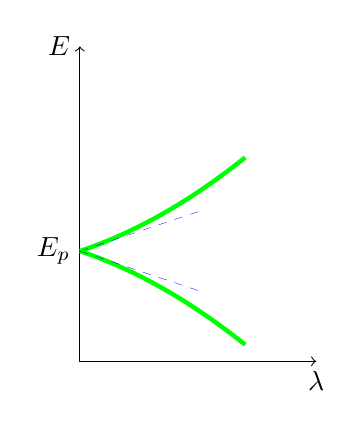
\begin{tikzpicture}[xscale=3,yscale=2]
    \draw [<->] (0,2) -- (0,0) -- (1,0);
    \draw[green, ultra thick, domain=0:0.7] plot (\x, {0.7+0.5*\x*\x + 0.5*\x});
    \draw[blue, ultra thin, dashed, domain=0:0.5] plot (\x, {0.7 + 0.5*\x});
    \draw[green, ultra thick, domain=0:0.7] plot (\x, {0.7-0.5*\x*\x - 0.5*\x});
    \draw[blue, ultra thin, dashed, domain=0:0.5] plot (\x, {0.7 - 0.5*\x});
    \draw node [left] at (0,0.7) {$E_p$};
    \draw node [left] at (0,2) {$E$};
    \draw node [below] at (1,0) {$\lambda$};
  \end{tikzpicture}
  \begin{tikzpicture}[xscale=3,yscale=2]
    \draw [<->] (0,2) -- (0,0) -- (1,0);
    \draw[green, ultra thick, domain=0:0.3] plot (\x, {0.7+ 0.5*\x});
    \draw[green, ultra thick, domain=0:0.3] (0.3,0.85) to [out=26.5,in=250] (0.7,1.5);
    \draw[green, ultra thick, domain=0:0.3] (0.3,0.85) to [out=26.5,in=-250] (0.7,0.5);
    \draw[blue, ultra thin, dashed, domain=0:0.3] plot (\x, {0.7 + 0.5*\x});
    \draw node [left] at (0,0.7) {$E_p$};
    \draw node [left] at (0,2) {$E$};
    \draw node [below] at (1,0) {$\lambda$};
  \end{tikzpicture}
  \caption{Los estados degenerados pueden desacoplarse al considerar
    perturbaciones en el hamiltoniano de orden suficiente. Se muestra también la
    aproximación lineal $E \sim E_p + \lambda \varepsilon_1$ en línea
    discontínua para ambos ejemplos.}
  \label{fig:uncoupling}
\end{figure}


En resumen, el procedimento se reduce a calcular la restricción de la
matriz $W$ en el subespacio de degeneración y diagonalizarla.
Los autovalores son las correcciones de primer orden a la energía, y
los autovalores dan los coeficientes de $\ket{0}$.

\subsection{Estructura fina del átomo de hidrógeno}
Aplicando la relatividad especial a la ecuación de Schrödinger se
puede obtener la ecuación de Dirac, cuyo hamiltoniano es:
\begin{equation}
  \begin{split}
     \Ham _\text{Dirac} &= mc^2 + \frac{p^2}{2m} + V(r) {}-{} \\ &-
    \underbrace{\frac{p^4}{8m^3c^2}}_{\text{mass}} +
    \underbrace{\frac{1}{2m^2c^2}\frac{1}{r}\dv{V}{r}\boldrm{l}\cdot
      \boldrm{s}}_{\text{spin-orbit}} +
    \underbrace{\frac{h^2}{8m^3c^2}\nabla^2V(r)}_{\text{Darwin}}
  \end{split}
\end{equation}
donde $m$ es la masa del electrón (\SI{9e-31}{\kilo\gram}). Los
términos de corrección, como se verá a continuación, tienen
aproximadamente el mismo valor y por tanto han de considerarse todos a
la vez.

\subsection{Término de masa}
La energía de una partícula libre es
\begin{equation}
  E = \sqrt{(pc)^2 + (mc^2)^2} = mc^2 \left[ 1 + \left( \frac{p}{mc} \right)^2 \right]^{\oh}
\end{equation}
Como $p \ll mc$ podemos efectuar un desarrollo de Taylor, obteniendo
\begin{equation}
  E = mc^2 + \frac{p^2}{2m} - \frac{1}{8} \frac{p^4}{m^3c^2}
\end{equation}
Obtenemos un nuevo término $W_m$, que corrige a la energía en reposo
($mc^2$) y al término cinético clásico ($\nicefrac{p^2}{2m}$).

Nos preguntamos si el término es despreciable frente a $ \Ham _0
= \frac{p^2}{2m} + V(r)$ en el átomo de hidrógeno. El
valor relativo del término se halla calculando
$\frac{W_m}{ \Ham _0}$, lo que nos da un valor
\begin{equation}
  \frac{W_m}{ \Ham _0} \sim
  \frac{\frac{p^4}{8m^3c^2}}{\frac{p^2}{2m}} = \frac{p^2}{4m^2c^2} =
  \frac{1}{4} \left( \frac{v}{c} \right)^2 \sim \alpha^2
\end{equation}
donde se ha utilizado el teorema del virial para afirmar que la
energía potencial de una partícula en un potencial central es del mismo orden de
magnitud que su energía cinética. El término $\alpha$, de valor
aproximado $\nicefrac{1}{137}$, es la \emph{constante de estructura fina}.

\subsection{Término de espín-órbita}
El electrón se mueve con velocidad $\boldrm{v}$ en el campo eléctrico
creado por el protón, que está situado a una distancia $r$. En el sistema de referencia del electrón existe
una espira con corriente (el proton que lo orbita) que genera un campo
magnético. Su valor en la posición del electrón es el de un dipolo magnético:
\begin{equation}
\boldrm{B}= \frac{\mu_0}{4\pi} e \frac{\boldrm{v}\times
  \boldrm{r}}{r^3} = \frac{-1}{c^2} \boldrm{v}\times \boldrm{E}
\end{equation}
donde $e > 0$ es el módulo de la carga del electrón, $c = (\mu_0
\varepsilon_0)^{-1/2}$ la velocidad de la luz en el vacío y $\boldrm{E} =
-k e \frac{\boldrm{r}}{r^3}$ el campo eléctrico que genera el protón.
Como el electron posee un momento magnético intrínseco
$\boldrm{M}_S$ de valor $e/m \cdot \boldrm{s}$ interactúa con el campo
magnético. Podemos escribir la energía de interacción como
\begin{equation}
  W_{\text{SO}} = - \boldrm{M}_S \cdot \boldrm{B}
\end{equation}
Escribamos el término de manera más explícita. El campo
electroestático $\boldrm{E}$ del protón se puede escribir como
\begin{equation}
  \boldrm{E} = \frac{-1}{e} \dv{V(r)}{r} \frac{\boldrm{r}}{r}
\end{equation}
donde $V(r) = \frac{-e^2}{r}$ es la energía electroestática del
electrón. Obtenemos:
\begin{equation}
  \begin{split}
    \boldrm{B} &= \frac{-1}{ec^2r} \dv{V(r)}{r} \boldrm{v}\times
    \boldrm{r} = \frac{-1}{mec^2 }\cdot \frac{1}{r}\dv{V(r)}{r}
    \boldrm{p}\times{\boldrm{r}} = \\ &= \frac{-1}{mec^2 }\cdot \frac{1}{r}\dv{V(r)}{r}
    \ \boldrm{l}
  \end{split}
\end{equation}
donde $\boldrm{l} = \boldrm{p}\times \boldrm{v}$ es el operador
momento angular. Obtenemos para el factor de corrección $W'$ un valor
\begin{equation}
  W_\text{SO} = \frac{1}{m^2c^2}\frac{1}{r}\dv{V(r)}{r} \boldrm{l}\cdot \boldrm{s}
\end{equation}
que corresponde con el término de espín-orbita salvo por un
factor\footnote{Because physics.} con valor aproximado $\oh$.

La corrección de este término también es aproximadamente $\alpha^2$.
Utilizando que $ \Ham _0$ es del orden de
$\frac{1}{4\pi\varepsilon_0} \frac{e^2}{r}$, y que
$\boldrm{l},\boldrm{s}$ son del orden de $\hbar$,
\begin{equation}
  \frac{W_{\text{SO}}}{ \Ham _0} \sim \frac{\frac{e^2
      \hbar^2}{m^2c^2r^3}}{\frac{e^2}{4\pi \varepsilon_0}\frac{1}{r}} = \frac{4\pi\varepsilon_0\hbar^2}{m^2c^2r^2}
\end{equation}
$r$ es del orden del radio de Bohr, $a_0 = 4\pi\varepsilon_0\hbar^2/me^2$. Obtenemos
\begin{equation}
 \frac{W_{\text{SO}}}{ \Ham _0} \sim \frac{1}{4\pi\varepsilon_0}\frac{e^4}{\hbar^2c^2}=\alpha^2
\end{equation}

\subsection{Término de Darwin}
Este término\historynote{Nombrado tras Sir Charles Galton Darwin
    (1887 – 1962), físico inglés nieto de Charles Darwin.} $W_D$ no tiene ninguna analogía clásica, y es puramente
cuántico. Para ver su orden de magnitud, utilicemos que $V(r)$ es un
potencial de Coulomb. Por tanto, la laplaciana del potencial será
proporcional a $\nabla^2(\nicefrac{1}{r})=-4\pi\delta(\boldrm{r})$,
luego
\begin{equation}
  \frac{\hbar^2}{8m^2c^2} \nabla^2V(r) =
  \frac{\hbar^2}{8m^2c^2}\frac{e^2}{4\pi\varepsilon_0}4\pi\delta(\boldrm{r})
  = \frac{\hbar e^2}{8m^2c^2\varepsilon_0}\delta(\boldrm{r})
\end{equation}
Cuando calculamos la media de este término en un estado atómico
genérico, obtenemos
\begin{equation}
  W_D = \bra{\psi(\boldrm{r})} W_D \ket{\psi(\boldrm{r})} =
  \frac{\hbar e^2}{8m^2c^2\varepsilon_0} |\psi(\boldrm{0})|^2
\end{equation}
Vemos que es proporcional a la función de ondas en el origen, por lo
que solo puede afectar a electrones de tipo \emph{s} (son los únicos
con $\psi\neq 0$ en el origen). El orden de magnitud de $|\psi(\boldrm{0})|^2$
puede hallarse integrando $|\psi(\boldrm{r})|^2$ sobre un volumen
acotado por $a_0^3$ e imponiendo que ello sea igual a 1, obteniendo
\begin{equation}
  |\psi(\boldrm{0})|^2 \sim \frac{1}{a_0^3}
\end{equation}
con lo que obtenemos que $W_D \sim \left( \frac{1}{4\pi\varepsilon_0}
\right)^3 \frac{me^8}{8c^2 \hbar^2 \varepsilon_0}$. Dividiendo entre
$ \Ham _0$, obtenemos $\frac{W_D}{ \Ham _0} = \alpha^2$. 

\section{Método variacional}
Sean un hamiltoniano $ \Ham $ con autoestados $u_E$ definidos por
\begin{equation}
   \Ham  u_E = E  u_E
\end{equation}
Puedo expresar cada función de ondas como
\begin{equation}
  \psi = \sum_{\{E\}} A_E u_E
\end{equation}
El valor medio de la energía es
\begin{equation}
  \ev{ \Ham }{\psi} = \sum_{\{E\}} |A_E|^2 E
\end{equation}
La energía del nivel fundamental cumple que $E_0 \leq E,\ \forall E$.
Por tanto
\begin{equation}
  \ev{ \Ham }{\psi} \leq E_0 \sum_{\{E\}} |A_E|^2 = E_0 \braket{\psi}{\psi}
\end{equation}
De forma que obtenemos
\begin{equation}
  E_0 \leq \frac{\ev{ \Ham }{\psi}}{\braket{\psi}{\psi}}
\end{equation}
Si escojo una $\psi \sim \psi_0$, obtendré un valor muy cercano a
$E_0$. De esta forma, obtengo un método para ajustar una función de
prueba $\psi_p(\alpha)$ de forma que se acerque lo máximo posible a
$\psi_0$, sólo tengo que minimizar $\ev{ \Ham }{\psi}$.

%%% Local Variables:
%%% mode: latex
%%% TeX-master: "../resumen"
%%% End:
